During the past 25 years a wide range of new ideas have been proposed for electricity point forecasting and for probabilistic forecasting. The field benefitted greatly from the increase of computing power, the greater availability of data and the interest in data science. As a consequence, the forecaster's toolbox has grown in size and complexity. Before delving into the literature review, we stress that at this point in time there is no superior method. Different solutions may outperform or underperform compared to other techniques depending on the problem settings. Thus, understanding the complexity, strengths and weaknesses of each method is crucial for fitting the right model to the right setting. Within this research community, the need for more homogeneity in the choice of the error valuation metrics emerged, see Section \ref{metrics}, along with the need of higher data quality and uniformity in the way of comparing model performances \cite{EPF_review}. As a solution, \cite{lago} proposes a checklist to aid evaluating the meaningfulness of new research. Throughout this thesis work, we will stick to the proposed principles and best practices peculiar of the EF field.
%literature review

\section{Electricity forecasting classification}
Electricity forecasting is a vague term and is used in the literature to refer to the whole field. Thus, in order to introduce some clarity, it is useful to classify the range of EF articles in terms of their core attributes.
In the context of energy forecasting, the quantities of most interest are electricity prices (EPF), electricity loads (ELF) and renewables generation (mostly wind and solar).
In terms of forecasting horizons, we can group EF into four major categories: very short term forecasting (VSTF), short term forecasting (STF), medium term forecasting (MTF) and long term forecasting (LTF). Consensus in the literature is to use one day, two weeks and three years respectively as cut off horizons \cite{hong_phd}; see Figure \ref{fig:time} for a visualisation. 
\begin{figure}
  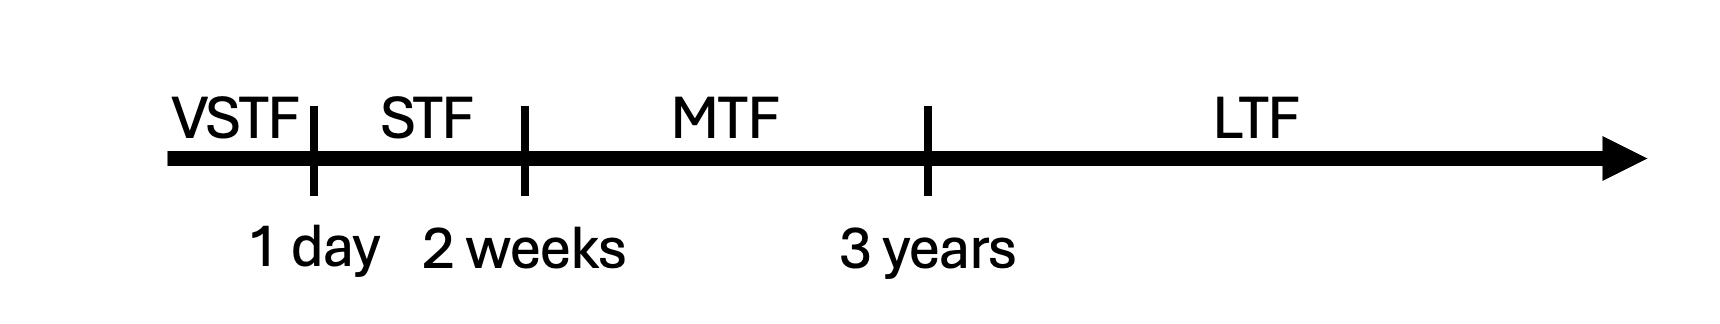
\includegraphics[width=\textwidth]{images/time_2.png}
  \caption{Time classification \cite{prob_elf}}
  \label{fig:time}
\end{figure}
Forecasts can either be for the whole target electricity network (system) or for a subset of it (zonal).
EF literature distinguishes between point and probabilistic forecasts. Each of the two has its advantages and disadvantages. Point forecasts are easier to generate and less computationally intensive while probabilistic forecasts are more informative. Industry and research efforts have focused primarily on point forecasting. Nevertheless, interest in probabilistic forecasting has risen considerably over the last years due to renewable integration requirements, introduction of smart grids and increased market competitiveness.
\section{Bibliographic analysis}
This section presents the results of the bibliometric analysis we performed on March $6^{th}$ 2024. This survey has been carried out by using the Scopus citation database. For details on the specific queries entered in Scopus, refer to Appendix \ref{src_code}.

To get started, let us consider the evolution of the EF field over the years. This is visualised in Figure \ref{fig:epf_evolution}, with results grouped by category. Articles prior to the 2000 have been aggregated together due to their small number. Figure \ref{fig:epf_evolution} shows the trend of an increasing interest in EF.
\begin{figure}
    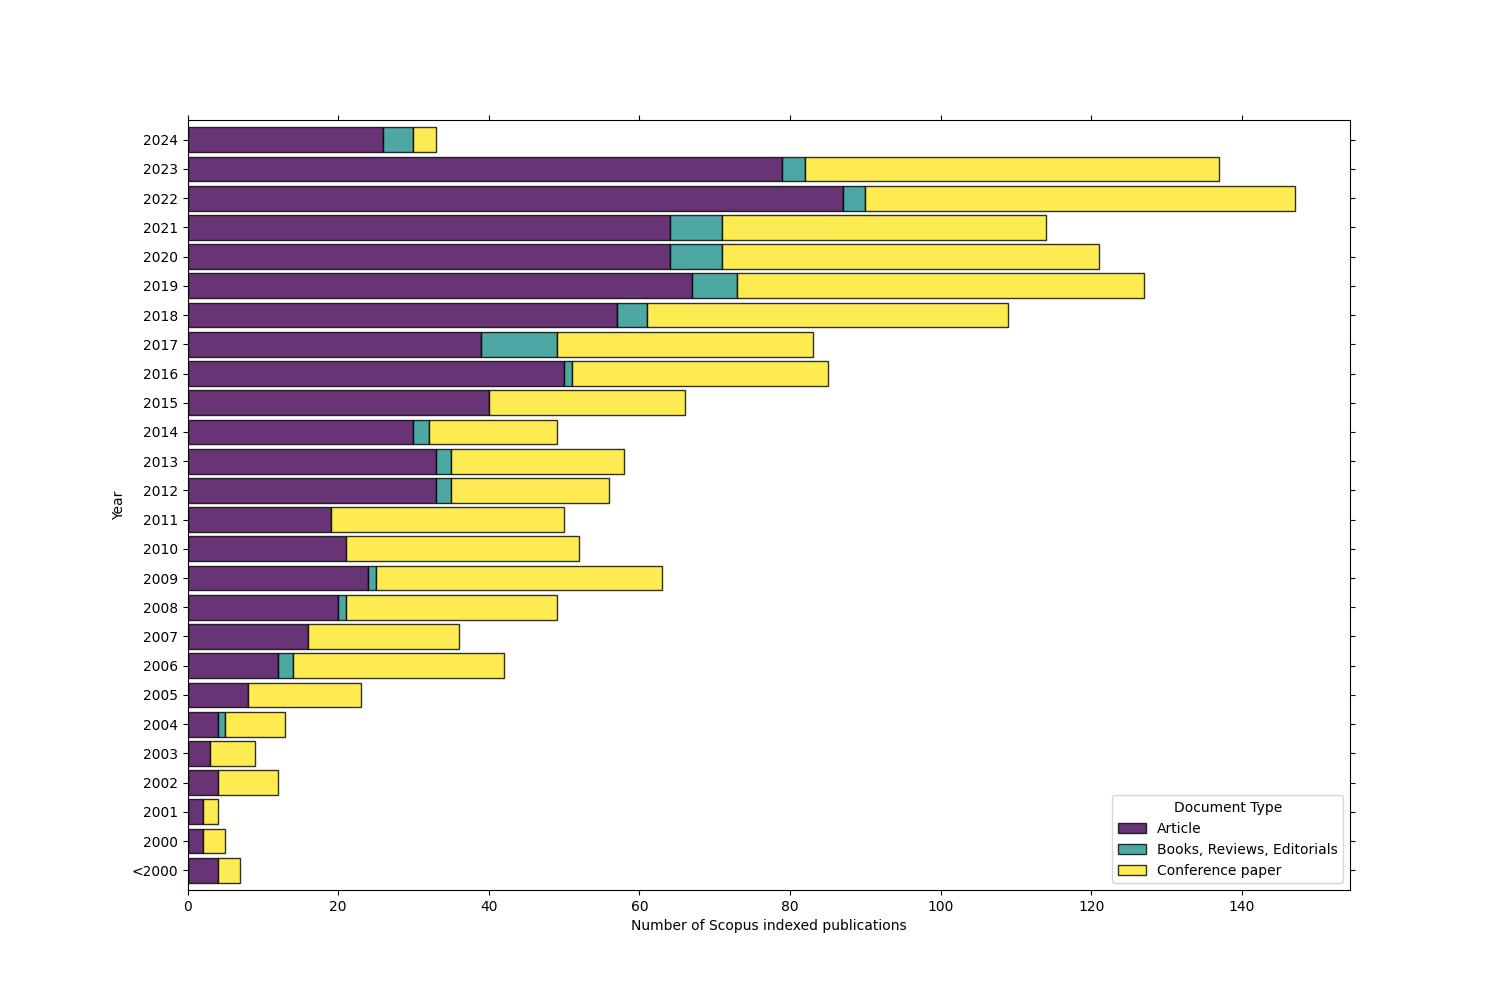
\includegraphics[width=\textwidth]{images/epf_evolution1.jpg}
    \caption{Electricity forecasting publications over the past years}
    \label{fig:epf_evolution}
  \end{figure}

The next question is to compare the state of point-versus probabilistic forecasting, this is visualised in Figure \ref{fig:point_vs_prob}. What can be concluded is that probabilistic-is less developed than point forecasting. To our mind this is due to the complexity of probabilistic forecasts.
Nevertheless, we can see a trend that suggests researchers are making an effort to fill this gap.

\begin{figure}
  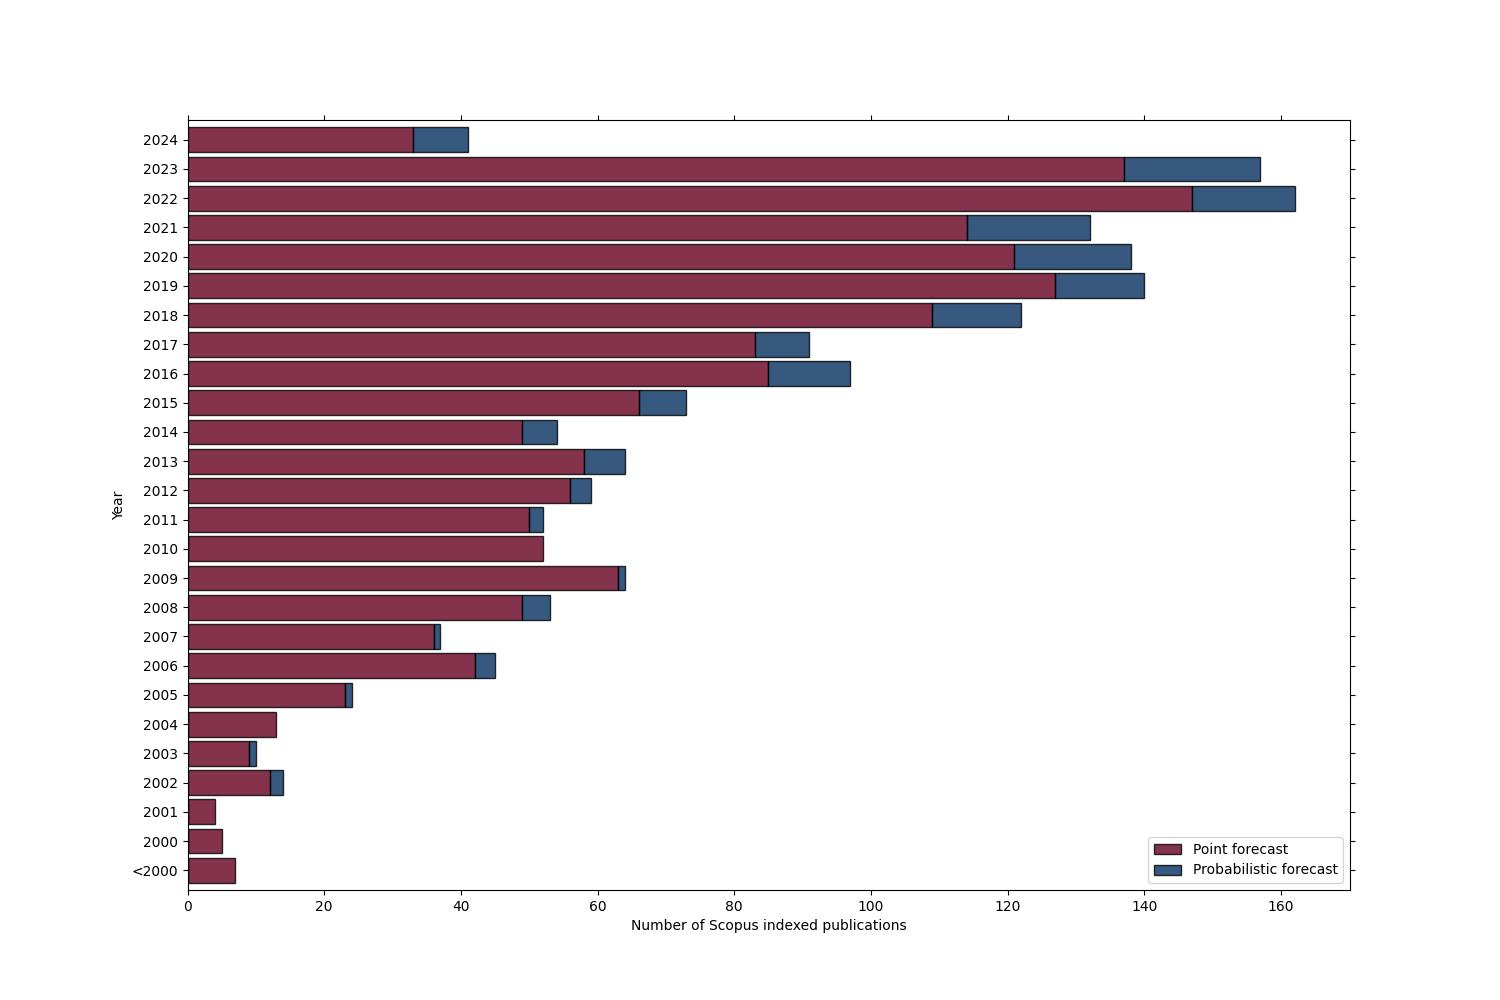
\includegraphics[width=\textwidth]{images/point_vs_prob.jpg}
  \caption{Point versus probabilistic publications over the past years}
  \label{fig:point_vs_prob}
\end{figure}

The EF literature is dominated by statistical-and computational intelligence (CI) methods as can be seen from Figure \ref{fig:cs_stat_both}, with CI methods being slightly preferred. 
\begin{figure}
  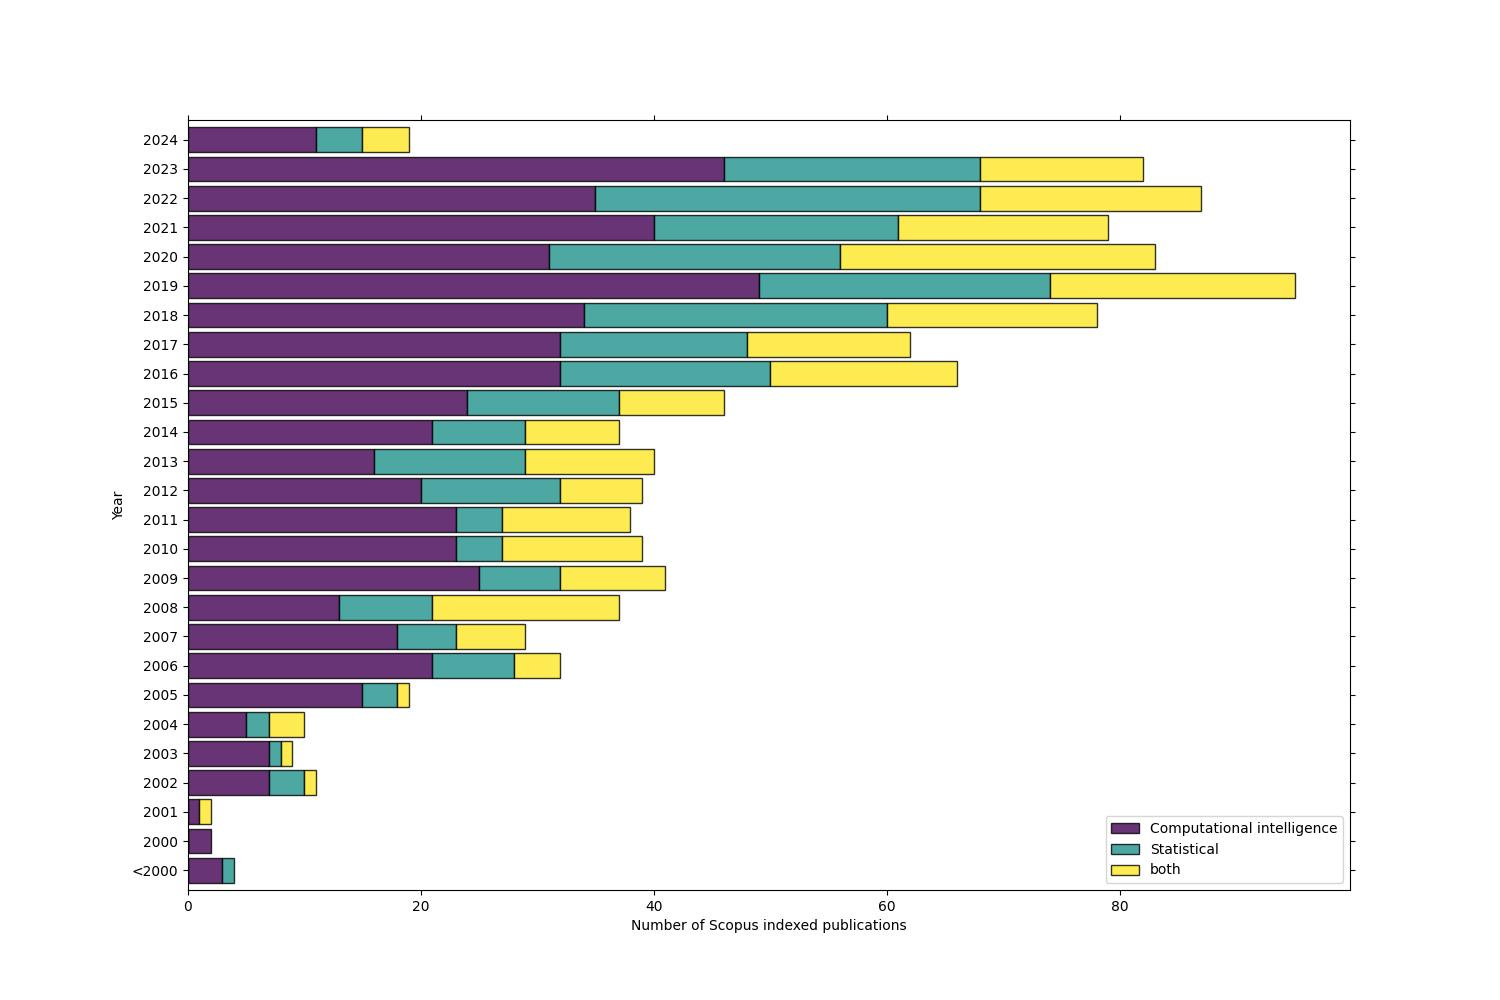
\includegraphics[width=\textwidth]{images/cs_stat_both.jpg}
  \caption{Publications by method over the past years}
  \label{fig:cs_stat_both}
\end{figure}

EF is a heterogeneous field of research, its researchers come from a wide array of backgrounds, with electrical engineers and statisticians making up the top contributors; their different educational training may explain why the split between statistical and computational intelligence methods is so marked. Figure \ref{fig:subject_area} depicts the EF publications by subject area. What can be concluded is that the bulk of publications come from engineering, computer science, mathematics and econometrics.
\begin{figure}
  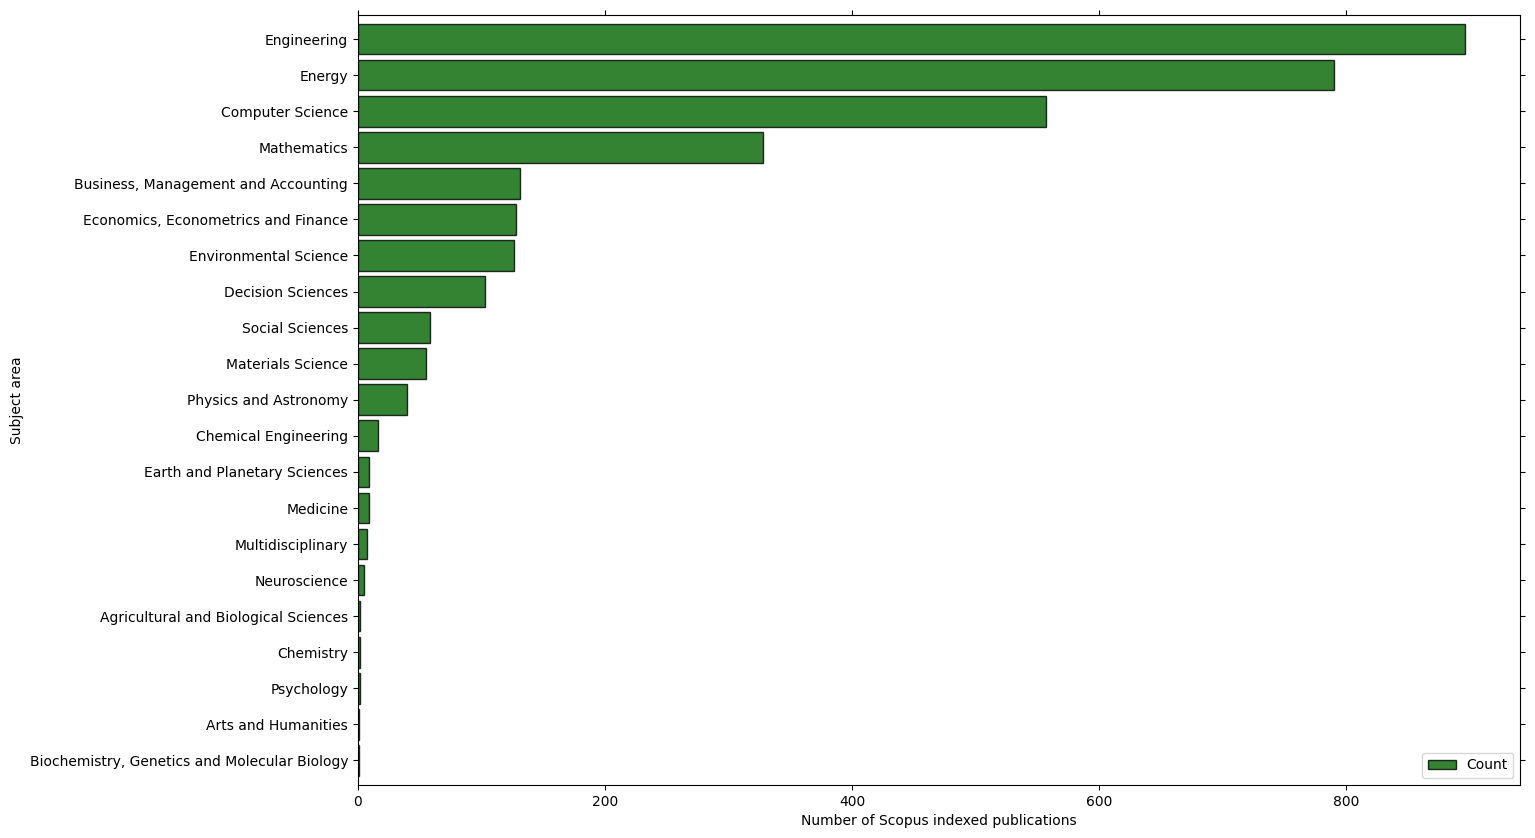
\includegraphics[width=\textwidth]{images/subject_area.png}
  \caption{Publications by subject area}
  \label{fig:subject_area}
\end{figure}

In order to refer to the most relevant source in the field, EF outlets have been ranked by popularity and plotted in Figure \ref{fig:src_title}.
\begin{figure}
  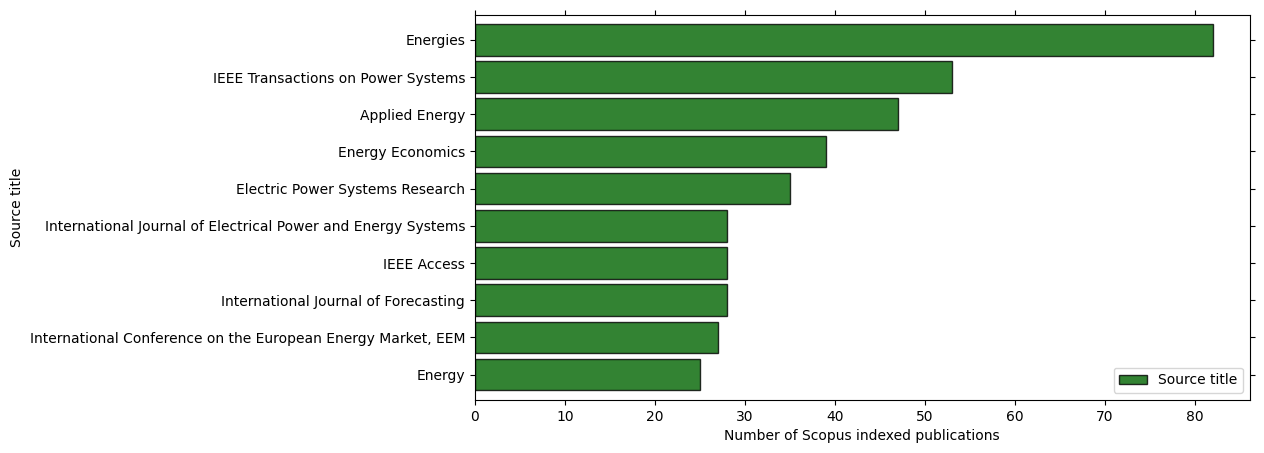
\includegraphics[width=\textwidth]{images/src_title.png}
  \caption{Most popular sources/outlets}
  \label{fig:src_title}
\end{figure}

\section{Electricity forecasting literature review}
To get started, a few review articles were collected in order to understand conventions, best practicies and terminology of the EF community.
Weron \cite{EPF_review} reviews the state of the art for electricity price forecasting. Besides analysing complexity of available solutions, strengths and weaknesses, it also stresses the need for objective comparative EPF studies. Specifically, it advocates for studies using similar datasets, using the same error evaluation metric and statistical testing model's outperformance.
Hong et al.\ \cite{prob_elf} discusses the state of the art in probabilistic electric load forecasting. It differentiates between techniques and methodologies. With techniques they refer to a family of models, like multiple linear regression or artificial neural networks. On the other hand, methodologies consist of general frameworks that can be incorporated into any method, for example variable selection mechanisms. Also this paper stresses the need for some guidelines to standardise research in the field.
Nowotarski et al.\ \cite{nowotarski} carried out a review of probabilistic forecasting.
Weron et al.\ \cite{lago} offer a set of best practices when forecasting electricity prices in order to have a common framework to evaluate and compare future research.
Zhang et al.\ \cite{zhang2014review} considers state of the art methods in wind power probabilistic forecasting and describes current challenges and possible future developments.
Ziel et al.\ \cite{ziel2018probabilistic} provides detailed tables, groups research papers by the time dimension and objective and reports datasets, models and accuracy 
measures adopted.
David et al.\ \cite{david2016probabilistic} adopts a combination of autoregressive moving average (ARMA) and generalised autoregressive conditional heteroskedasticity (GARCH) in probabilistic forecasts of solar irradiance. Furthermore, they propose a recursive framework for parameter estimation.
De Gooijer \cite{de200625} reviews 25 years of time series forecasting for the period 1990-2005, highlighting the most influential works.
He et al.\ \cite{he2022cooperative} models multistep wind speed probabilistic forecasting by mixing complementary ensemble empirical mode decomposition (CEEDMAN), least absolute shrinkage and selection operator (LASSO) and quantile regression (QR). In this work, CEEMDAN is used to decompose the wind speed time series, LASSO compresses high dimensional features, QR is used for obtaining quantile forecasts, finally kernel density estimation (KDE) converts quantile forecasts into density estimates.
Wan et al.\ \cite{wan2016direct} proposes a combination of QR and extreme learning machine (ELM) to generate non parametric probabilistic forecasts of wind generation.
Zhang et al.\ \cite{zhang2019wind} forecasts wind speed by adopting QRMGM, which is a combination of QR with a minimal gated memory network.
Hyndman et al.\ \cite{hyndman1996estimating} explains kernel estimator of conditional density, analyses its asymptotic behaviour and covers an application for the daily temperatures of Melbourne.
Kaur et al.\ \cite{kaur2022energy} carries out a comparative study of techniques spanning ideas from statistics and artificial intelligence.
Van der Meer et al.\ \cite{van2018review} provides another thorough analysis of the probabilistic forecasting realm by covering recent advances and identifying research gaps.
The IEEE Power and Energy Society provides also insightful lecture notes on probabilistic energy forecasting methodologies,
implementations, and applications \citeW{gm_22}.
Marcjasz et al.\ \cite{probablistic_electricity_forecast2} uses distributional neural networks to create probabilistic forecasts for the day ahead electricity prices in the German market.
Nowotarski et al.\ \cite{nowotarski2015computing} introduce a method for constructing prediction intervals (PI) and call it quantile regression averaging. Their idea is weighting a set of model predictions such that the pinball loss of the weighted model is minimised. The observed result is that QRA performed better compared to twelve individual models.
Arora et al.\ \cite{arora2016forecasting} focus on modelling electricity smart meter data by proposing a non parametric probabilistic technique based on kernel density estimation and conditional kernel density estimation \cite{rosenblatt1969conditional, hyndman1996estimating}. Their conclusion is that kernel density methods are competitive against exponential smoothing when forecasting residential data. Conversely, exponential smoothing has still an edge in predicting small to medium-sized enterprises data (SMEs).
Zhang et al.\ \cite{zhang2020probability} introduce a framework based on quantile regression and kernel density estimation in the context of short term wind forecasting. The proposed methods behave well compared to an autoregressive ARMA model.
% ARMA(p=1,q=1) 
Haben et al.\ \cite{haben2018short} analyses a variety of techniques in terms of both probabilistic and point forecasting. Within this study, they focus on load forecasting at the low voltage level.
%Metrics Start
Koochali et al.\ \cite{koochali2022random} reviews various existing methods for assessing probabilistic forecast models and discusses their advantages and disadvantages.
Matheson et al.\ \cite{matheson1976scoring} develops classes of scoring rules for continuous probability distributions.
Gneiting et al.\ \cite{gneiting2007strictly}
provides a thorough overview of the theory of scoring rules for interval and density forecasts.
Gneiting et al.\ \cite{gneiting2014probabilistic}
covers theory and state of the art techniques in probabilistic forecasting.
%Metrics End
Zhang et al.\ \cite{zhang2020two} proposes a two stage bootstrap sampling framework for probabilistic load forecasting. They test it for different regression models such as random forest (RF), gradient boosting regression tree (GBRT), linear regression, and least squares support vector regression (LSSVM).
Jónsson et al.\ \cite{jonsson2014predictive}
introduces a density model for the day ahead market extending the adaptive QR framework of \cite{moller2008time} by modelling the tails of the predicted density with an exponential distribution.
Fatema et al.\ \cite{fatema2023probabilistic} considers Gaussian process regression for point forecasting and prediction intervals estimation. Then, it inputs prediction intervals to kernel density estimation in order to estimate a probability distribution.
Dudek \cite{dudek2018probabilistic} proposes a probabilistic forecasting model based on the Nadaraya Watson estimator \cite{nadaraya1964estimating,watson1964smooth}.
Huurman et al.\ \cite{huurman2012power} surveys the predictive power of weather variables for electricity prices in the Danish market. Their empirical results suggest that weather is central for point forecasting day ahead prices. The opposite conclusion are drawn for density forecasting.
Lately, the idea of combining forecasts has gained popularity in the forecasting community \cite{forecasting_big}. In the literature, combined forecasts are called ensemble \cite{gneiting_weather_ensemble}.
Experimental results have shown ensemble methods to outperform their component forecasts.
Note that, the more the errors of the combined models are not correlated, the more we can benefit from ensembles.
It is also worth noting that older and simpler methods are still valuable (in combination with other models or on their own), these being less subject to overfitting than complex models.

%GEFCom2012
A major step forward in EF was the creation of the global energy forecasting competition (GEFCom) in 2012. Until then, no formal benchmarking process or data pool was established and new publications rarely reproduced the results from work done by others. Addressing these issues was the motivation behind the creation of GEFCom by the IEEE working group on energy forecasting. The EF field was positively affected by this competition. A number of ideas were tested on the same setting with only the best ones being published and it also contributed bridging the gap between industry practice and academic research. GEFCom2012 had two tracks; the former about hierarchical load forecasting, the latter about wind power forecasting, see \cite{hong2014global} for a comprehensive review. 
%GEFCom 2014
The focus of GEFCom2014 was on probabilistic forecasting, Hong et al.\ \cite{hong2016probabilistic} discusses the problem tracks, the data and the winning methods.
In this paragraph some of the winning entries of the 2014 GEFCom edition are discussed.
Xie et al.\ \cite{xie2016gefcom2014} proposes a two stage approach; in the first stage they use multiple linear regression (MLR) to build a point forecast, then in the second stage they try different approaches for modelling the MLR residuals, among other they tried exponential smoothing (ESM), artificial neural networks (ANN) and autoregressive integrated moving average (ARIMA). 
Maciejowska et al.\ \cite{maciejowska2016hybrid} proposes a new probabilistic model extending the idea of quantile regression averaging (QRA) \cite{nowotarski2015computing}.
Haben et al.\ \cite{haben2016hybrid} mixes conditional kernel density (CKD) and quantile regression in their competition entry.
Gaillard et al.\ \cite{gaillard2016additive,gaillardasemi} combines quantile regression with generalised additive models \cite{hastie2017generalized}.
Ziel et al.\ \cite{ziel2016lasso} estimates an AR model through the LASSO \cite{tibshirani1996regression} instead of the standard OLS.
%GEFCom 2017
The last GEFCom was held in 2017, its focus was providing hierarchical probabilistic load forecasts, see \cite{hong2019global}. The GEFCom competition has also inspired the organisation of other competitions such as the RWEnpower competition in the UK, the RTE competition in France, the Tokyo electric power company competition in Japan and the BigDEAL forecasting competitions.

A couple of considerations can be drawn from the above literature review.
The EF field is characterised by heterogeneity in its forecasting techniques; methods come from statisitics, mathematics, econometrics, electrical engineering and the artificial intelligence communities.
Every paper uses different datasets.
Therefore, it is not possible to directly compare results from one paper to another without implementing the paper specific algorithms and then applying them to the respective dataset. An additional hurdle is that some datasets are not freely accessible.
Thus, a good understanding of the state of the art methods in EF is required to carry out a rigorous comparison between methods.
That is why the following chapters are devoted to summarising the mathematical theory underlying such techniques.

\section{Kernel methods literature review}
%INTRO KERNEL METHODS E ENERGY PRICE MODELLING
Kernel methods are a class of algorithms for pattern analysis.
With kernel methods we are able to apply linear methods with predictors in a high dimensional space, without having to explicitly evaluate the involved dot products of the features.
Throughout this thesis, we will address the performance of kernel methods in the context of EF.

%- Kernel history evolution.
Their name comes from the German word kern, which translates to core in english. Such term was first used by David Hilbert in his paper on integral equations \cite{hilbert} where he introduced the term "definite kernels". Following, Hilbert's and Schmidt's work, \cite{schmidt} lead to the introduction of a new space, the Hilbert space.
In 1909, James Mercer improved Hilbert's work by proposing his theorem \cite{mercer}. This theorem underlies the power of kernel methods, that is the kernel trick.
In 1938, Schoenberg \cite{schoenberg} developed the mathematical results that allow us to find the kernel associated to a specific feature space metric.
In 1941, Kolmogorov \cite{kolmogorov} carried out stuides on representing kernels in linear spaces.
In 1950, Aronszajn \cite{aronszajn} published the first work on reproducing kernel Hilbert spaces (RKHS); developing the general method for representing kernels in linear spaces.
In 1964, Aizerman \cite{aizerman} further improved the theory of RKHS.
It was in the 1990s that the theory of kernel methods got popular, particularly in the field of machine learning. Kernels have been used in various different tasks such as support vector machines (SVM) \cite{vapnik1, vapnik2}, Gaussian process classifiers \cite{williams}, spline methods \cite{wahba}, neural networks \cite{poggio} and principal component analysis \cite{pca_scholkopf}.
Nevertheless kernel methods received very little attention in the specific setting of EF literature.

The kernel theory needed for this thesis work is covered in Section \ref{kernel_theory}. 
For an introduction to kernel methods, we refer to \cite{learning_with_kernels, hofmann2006review, shawe2004kernel}.

Kanagawa et Fukumizu introduces to the concept of kernel mean embedding \cite{pmlr}. Muandet et al.\ \cite{Muandet_2017} surveys established results and new advances in the theory of Hilbert space distribution embeddings. 
It has to be said that, computing and storing such embeddings becomes prohibitive for large scale settings. Rudi et al.\ \cite{2022nystrom} proposes an efficient approximation procedure based on the Nyström method \cite{nystrom}, providing also an upper bound for the approximation error.
Another example of the applicability of kernel methods is \cite{supersamples}. In that paper, Smola et al.\ kernelize the herding algorithm introduced in \cite{welling2009herding,welling2009herding,Welling2010}. The original herding algorithm converts empirical moments into a sequence of pseudo-samples approximating the probability density function (PDF) of the observed random variable. Its weakness is that it can only take a finite number of features and this limits its expressive power.
Smola et al.\ overcomes this by translating the algorithm into the framework of kernels.

% Smola et al. \cite{supersamples} presents kernel herding; basically, the authores used the kernel trick to extend the herding algorithm to continous spaces. The result is an infinite memory deterministic process that takes in a collection of samples and learns to approximate a probability density function (PDF).

%QUESTO DA VEDERE
% Particularly extending the idea of \cite{2022nystrom}, where the Nyström approximation is employed in computing the kernel mean embedding, experiments with the Pivoted Cholesky decomposition will be performed.